\documentclass{article}
\usepackage[utf8]{inputenc}
\usepackage[margin=1.5in]{geometry}

\usepackage{graphicx}
\usepackage{amsmath}
\usepackage{braket}
\usepackage{parskip}
\usepackage{hyperref}

\usepackage{listings}
\usepackage[usenames,dvipsnames]{color}

\lstset{ 
    language=R,                       % the language of the code
    basicstyle=\small\ttfamily,       % the size of the fonts that are used for the code
    numbers=left,                     % where to put the line-numbers
    numberstyle=\tiny\color{Blue},    % the style that is used for the line-numbers
    stepnumber=1,                     % the step between two line-numbers. If it is 1, each line will be numbered
    numbersep=5pt,                    % how far the line-numbers are from the code
    backgroundcolor=\color{white},    % choose the background color. You must add \usepackage{color}
    showspaces=false,                 % show spaces adding particular underscores
    showstringspaces=false,           % underline spaces within strings
    showtabs=false,                   % show tabs within strings adding particular underscores
    numbers=none,                     % no line numbers
    frame=single,                     % adds a frame around the code
    rulecolor=\color{black},          % if not set, the frame-color may be changed on line-breaks within not-black text (e.g. commens (green here))
    tabsize=2,                        % sets default tabsize to 2 spaces
    captionpos=b,                     % sets the caption-position to bottom
    breaklines=true,                  % sets automatic line breaking
    breakatwhitespace=false,          % sets if automatic breaks should only happen at whitespace
    keywordstyle=\color{RoyalBlue},   % keyword style
    commentstyle=\color{YellowGreen}, % comment style
    stringstyle=\color{ForestGreen}   % string literal style
} 

\title{Final Project Report \\ \large Scientific Computation and Programming}
\author{Connor Broyles}
\date{December 2020}

\begin{document}

\maketitle

\section{Introduction}
The field of quantum computing has expanded drastically over recent years. Quantum computers can exponentially accelerate certain types of calculations, making them a promising candidate for some applications, especially as classical computers start to see complicated physical barriers to their improvement.

This project introduces Quantal: an environment for experimentation with quantum computing. This project is composed of two main components to aid in its goal: an R library for quantum computing, and a Shiny web application that can be used to write quantum programs and view their output. As the mathematics behind quantum computing heavily utilize linear algebra and statistics, R is an excellent platform for simulating quantum computing.

The quantum computing library provides the basic tools for quantum computing, such as a qubit object and the common quantum gates. A quantum circuit construct is implemented upon these building blocks. This circuit can have an arbitrary number of qubits, specified by the user, and supports operations for all of the gates defined by the library. New gates can be easily implemented if desired.

The Shiny application provides an environment in which to write simple quantum programs. It consists of a code editor, a circuit diagram viewer, and plots of the circuit's state vector and state probabilities.

The source code for Quantal is hosted at the following location: \url{https://github.com/cbrl/Quantal}


\section{Implementation}
\subsection{Quantum Computing Library}
\subsubsection{Low-Level Components}
The low-level components of the library include a set of primitives such as the qubit and quantum gates. The components can be used directly if desired, but are more powerful when used as part of the higher-level quantum circuit components.

Qubits and gates are implemented using the built-in matrix functionality within R. This allows the library to easily take advantage of R's extensive standard library features for working with matrices. A qubit's state vector is just a standard matrix of complex numbers behind the scenes, as is a quantum gate. Therefore, a gate can be applied to a qubit using the same matrix multiplication operator that an R user is familiar with, as seen in the example below.

\vspace{1em}

\begin{lstlisting}[caption={Applying a Hadamard gate to $\ket{0}$}]
> H %*% ket(1, 0) #alternatively: H %*% as.qubit(0)
             [,1]
[1,] 0.7071068+0i
[2,] 0.7071068+0i
\end{lstlisting}

\subsubsection{Quantum Circuit Components}
The quantum circuit builds on the basic quantum computing components. It contains the state of a circuit with an arbitrary number of qubits, specified by the user. The user can then execute a series of operations on the circuit. Internally, these operations are stored in a list, to later be compiled when requested by the user. The quantum circuit compiles the instructions into a single unitary gate which acts on the circuit's statevector.

The following example demonstrates the creation of Bell state on a 2-qubit quantum circuit:

\begin{lstlisting}[caption={Bell state on a 2-qubit quantum circuit}]
> cir <- qc.quantum_circuit(2) #quantum circuit with 4 qubits
> qc.h(cir, 1) #apply H gate to qubit 1
> qc.cx(cir, 1, 2) #CX gate with qubit 1 = control and 2 = target
> qc.compile(cir)
> qc.run(cir)
> basis_probs(cir$statevector) #prob. of measuring each basis state
$`00`
[1] 0.5

$`01`
[1] 0

$`10`
[1] 0

$`11`
[1] 0.5
\end{lstlisting}

Methods for applying a gate to a quantum circuit are provided for every library-provided gate. User-specified gates can be included as a drop-in addition, so long as they are compatible with the format used in the library.

The library includes a parser for a very basic quantum computing language, as seen in the Shiny application. Given a valid program, the parser will return a compiled quantum circuit with the gates specified by the program applied to it. The section below shows an example of the creation of a Bell state in the language:

\newpage

\begin{lstlisting}[caption={Bell state in quantum programming language}]
qubits 2
H  1
CX 1 2
\end{lstlisting}

A valid program starts with a "qubits N" line, where N is the number of qubits in the circuit. The following lines are instructions to execute. Each instruction is a gate name, followed by the qubits it acts on. In the case of the conditional gates, the first qubit is the control, and the second qubit is the target.


\subsection{Shiny Web Application}
The central part of this project is the Shiny web application. This application provides a graphical environment for experimenting with quantum computing. It can be separated into four main features: the code editor, the circuit diagram, the probability plot, and the state vector plot.

\begin{figure}[h!]
    \centering
    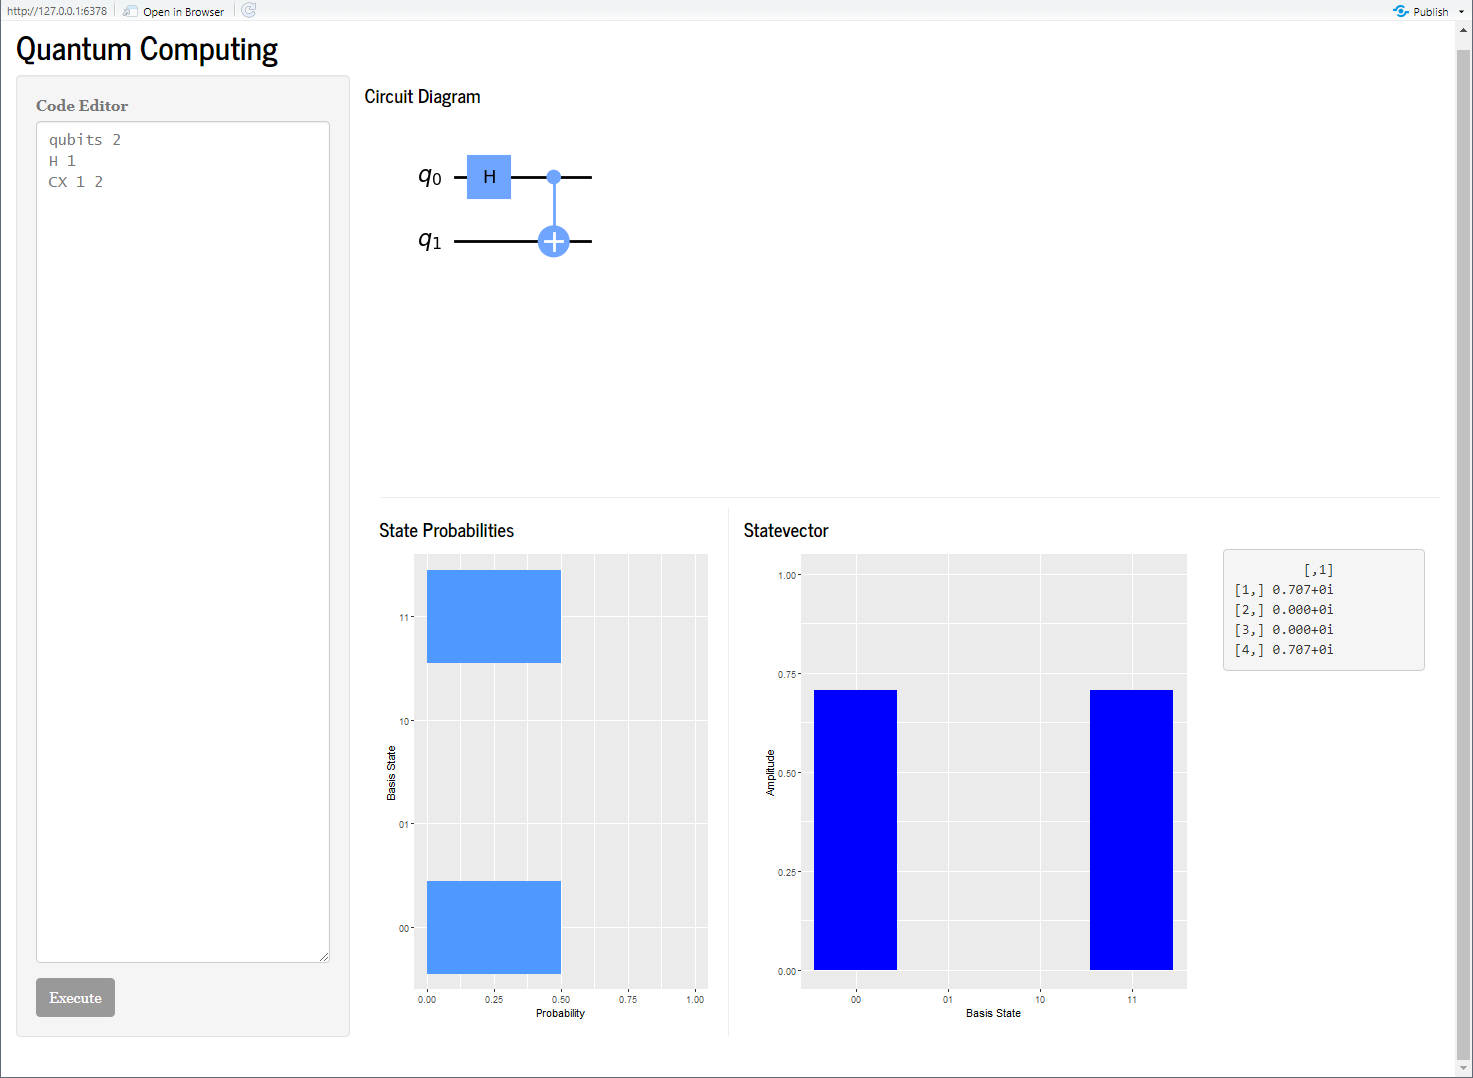
\includegraphics[width=\linewidth]{editor.png}
    \caption{A view of the Shiny application after running the Bell state program}
    \label{fig:shiny_app}
\end{figure}

\subsubsection{Code Editor}
The code editor is a basic text input box in which the user can write a program in the language discussed previously. At the bottom of the editor is an "Execute" button, which will parse the program, generate a circuit diagram, run the circuit, and display the output.

\subsubsection{Circuit Diagram}
The circuit diagram is generated whenever the user executes a quantum program. For this feature, the library utilizes the existing diagram generation feature of the popular Qiskit library. Interaction with Qiskit happens through the \textbf{reticulate} library in R.

\subsubsection{Probability Plot}
The probability plot displays the probability of measuring the system in each potential basis state after executing the program.

\subsubsection{State Vector Plot}
The state vector plot displays the absolute value of each probability amplitude in the quantum circuit's state vector. This of course removes the phase information from the value. The phase information is instead encoded as the color of the bar, which gives a quick visual indicator of differing phases in the state vector. In addition, the actual value of the state vector is displayed as a numeric array to the side of the plot.


\section{Future Work}
Quantum computing is an extremely complex subject. This project currently covers only the basics, and has significant room for expansion.

For the library, realistic circuit simulation is a good next step. The quantum circuit model assumes a perfect environment, which is of course unrealistic. An actual quantum circuit would have noise which interferes with measurement results. Simulating the effect of noise would make a big step towards a realistic circuit simulation.

The Shiny app has plenty of room for improvement. The user experience leaves much to be desired for real use. An improved UI and documentation would significantly boost its usefulness. More information about the quantum state could be displayed, such as a dedicated output for the phase portion of the circuit's state vector.


\section{Conclusions}
This project introduces Quantal: an environment for experimenting with quantum computing within the R language. The project's quantum computing library provides a quantum circuit construct, which builds on the library's low-level qubit and gate structures. The quantum circuit can either be interacted with directly, or constructed using the basic quantum programming included with the library. The Shiny web application incorporates these components into a graphical environment that allows the user to write a quantum program, view its representative circuit, and analyze the program's output.


\begin{thebibliography}{9}
\bibitem{ibm_quantum}
IBM Quantum Experience
\\\url{https://quantum-computing.ibm.com/}

\bibitem{qiskit_website}
Qiskit: Open Source Quantum Development
\\\url{https://qiskit.org/}

\bibitem{umass_quantum_tutorial}
Emma Strubell.
\textit{An Introduction to Quantum Algorithms}.
\\\url{https://people.cs.umass.edu/~strubell/doc/quantum_tutorial.pdf}
\end{thebibliography}

\end{document}
